% !TeX root = RJwrapper.tex
\title{cmcR: Congruent Matching Cells Method in R for Cartridge Case
Identification}
\author{by Joseph Zemmels, Susan VanderPlas, and Heike Hofmann}

\maketitle

\abstract{%
Scientific research is driven by our ability to use existing methods,
procedures, and materials from previous studies and further this
research by adding to it. As the need for computationally-intensive
methods to analyze large amount of data grows, the criteria needed to
achieve reproducibility, specifically computational reproducibility,
have become more sophisticated. In general, prosaic descriptions of
algorithms are not detailed or precise enough to ensure a complete
reproducibility of a method. Results may be sensitive to conditions not
commonly specified in written-word descriptions such as implicit
parameter settings or the programming language used. To achieve true
computational reproducibility, it is necessary to provide all
intermediate data and code used to produce published results. In this
paper, we consider a class of algorithms developed at the National
Institute of Standards and Technology (NIST) to perform firearm evidence
identification on cartridge case evidence known as the
\dfn{Congruent Matching Cells} (CMC) methods. To date, only textual
descriptions of these algorithms have been published. We introduce the
first open-source implementation of the Congruent Matching Cells methods
in the R package \CRANpkg{cmcR}. We have structured the \CRANpkg{cmcR}
package as a set of sequential, modularized functions intended to ease
the process of parameter experimentation. We use \CRANpkg{cmcR} and a
novel variance ratio statistic to explore the CMC methodology and
illustrate problems that arise when only computationally ambiguous
descriptions of algorithms are provided.
}

\hypertarget{intro}{%
\section{Introduction}\label{intro}}

\dfn{Research reproducibility} refers to the ability to use the same
procedures and materials as a previous study to arrive at the same
results or conclusions. Reproducibility is indispensable for results to
be considered valid by the wider scientific community
\citep{goodman_what_2016}. Unfortunately, we cannot take reproducibility
for granted: recent studies have raised concerns about reproducibility
of scientific findings in various fields
{[}\citet{king_replication_1995}, \citet{baker_1500_2016},
\citet{pasquier_if_2017}{]}. Commonly identified reasons for this lack
of reproducibility include (1) ambiguity in how procedures were
implemented, (2) missing or incomplete data, and (3) missing or
incomplete computer code to replicate all statistical analyses
\citep{leek_is_2017}.

In computational research, reproducibility of results is commonly
translated to mean that the code and data used to produce published
results be made publicly available \citep{peng_reproducible_2011}.
However, current status quo is that many papers describe the
computational methods used in the data analysis in broad terms only.
Computational reproducibility requires more details: published results
may be numerically sensitive to the particular implementation of a
computational method, including such considerations as data processing
decisions, parameter settings, and even the chosen programming language.
As such, peer-review and scientific progress in the truest sense
requires that \emph{all} pre-processed data, code, and results be made
openly available. In recognition of the additional requirements of
computational reproducibility, some journals have adopted policies
encouraging or requiring that authors provide code and data sufficient
to reproduce the statistical analyses, with the goal of building a
``culture of reproducibility'' in their respective fields
\citep{peng_reproducible_2009, peng_reproducible_2011, stodden_toward_2013}.

The fundamental reason that descriptions of data analysis procedures,
combined with the raw data, are not sufficient for reproducibility is
that published procedures are described in words rather than
algorithmically, and in some cases, steps are performed manually without
providing the resulting intermediary outcomes. If the written-language
description of the method in the publication is the sole source of
information about the algorithm, we trade computational reproducibility
for readability. We generally do not describe the particular parameter
settings used (or how those were derived) when we describe an algorithm
in a publication. This is an understandable editorial decision, as the
purpose of a publication is to demonstrate and justify the method rather
than discuss the fine details and parameter settings. Because
publications generally do not contain sufficient detail to reproduce
every part of the algorithm, it is necessary to supplement the paper
with open code and intermediate forms of the data (after any manual
steps have been performed or simply as check points for replications).
Especially in applications like forensic science or medicine, where
results from computational methods may directly affect an individual's
life, transparency in how a method or algorithm is implemented is
necessary \citep{angwin_machine_2016, cino_deploying_2018}.

In this light, computational reproducibility in forensic science, is all
the more important because it fundamentally enables discussions about
algorithmic transparency and accountability
\citep{kwongAlgorithmSaysYou2017, desaiTrustVerifyGuide2017}. Currently,
subjective decisions are made by individual examiners -- human beings
are the ultimate closed-source, black-box system, and the operations
which lead to a decision are largely opaque. The
\citet{council_strengthening_2009} has pushed to complement these
subjective decisions with automatic algorithms that objectively assess
evidence and can be explained during court testimony. It furthermore is
of the utmost importance that the community does not go only halfway,
trading a subjective, human black box for objective, proprietary
algorithms that are similarly opaque and unauditable. As part of the
shift towards objectivity in forensic science, automatic methods have
been developed to solve problems such as identifying matching glass
shards \citep{park2019}, handwriting \citep{crawford_handwriting_2020},
shoe prints \citep{park_algorithm_2020}, and ballistic evidence
\citep{hare_automatic_2016,tai_fully_2018}. However, many of the
algorithms described in the literature are not reproducible or
open-source. In this paper, we will demonstrate the ambiguities present
in textual descriptions of algorithms by creating an open-source
implementation of one well-known automatic forensic identification
method. The Congruent Matching Cells (CMC) algorithm was developed at
the National Institute of Standards and Technology (NIST) in 2012 to
perform firearm evidence identification using identifiable markings left
on spent cartridge cases from a firearm's barrel
\citep{song_proposed_2013}. Since then, the method and its numerous
extensions
\citep{tong_improved_2015,chen_convergence_2017,song_estimating_2018}
have shown promise in being able to differentiate between matching and
non-matching cartridge cases. While NIST researchers and collaborators
have been able to build on the foundation of the original algorithm, the
code and data necessary to reproduce the results have not been made
available to external researchers. As a result, the findings described
in those papers are not computationally reproducible for the research
community at large.

Here, we describe the process of implementing the Congruent Matching
Cells (CMC) method for the comparison of marks on spent cartridge cases,
using the descriptions from two published papers, \citet{song_3d_2014}
and \citet{tong_improved_2015}. Our R package, \CRANpkg{cmcR}, provides
an open-source implementation of the CMC method, but it also serves as
an example of the implementation barriers which occur when translating
textual descriptions of algorithms into detailed source code. This
process offers some insight into the necessary components which must be
available for computational reproducibility. Our experience shows that
when faced with ambiguity in how a method is implemented, there are few
options available to us apart from performing brute-force searches
through combinations of decisions that may have yielded the results
reported. Unsurprisingly, the process is both time absorbing and
computationally intensive from implementation to sifting through a wide
variety of decision combinations. The failure to ensure computational
reproducibility not only imposes a general barrier to scientific
progress; in this application, it also highlights the crucial need of
open-source, transparent methodology in high-stakes fields such as
forensic analysis.

We will use the same data set which is referenced in
\citet{song_3d_2014} and \citet{tong_improved_2015} to illustrate usage
of the \CRANpkg{cmcR} package. These 3D scans of cartridge cases are
available from the NIST Ballistics Toolmark Research Database
\citep[NBTRD;][]{nbtrd}. The strings defined below refer to three
cartridge case scans available on the NBTRD from
\citet{fadul_empirical_2011} and will be used throughout the remainder
of this paper.

\begin{Schunk}
\begin{Sinput}
library(cmcR)

nbtrd_url <- "https://tsapps.nist.gov/NRBTD/Studies/CartridgeMeasurement"

x3p_ids <- c("DownloadMeasurement/2d9cc51f-6f66-40a0-973a-a9292dbee36d",
             "DownloadMeasurement/cb296c98-39f5-46eb-abff-320a2f5568e8",
             "DownloadMeasurement/8ae0b86d-210a-41fd-ad75-8212f9522f96")

file_names <- c("fadul1-1.x3p","fadul1-2.x3p","fadul2-1.x3p")

purrr::walk2(.x = x3p_ids,
             .y = file_names,
             .f = function(x3p_id,file_name){
               download.file(url = file.path(nbtrd_url, x3p_id), 
                             destfile = paste0("data/",file_name),mode = "wb")
             })
\end{Sinput}
\end{Schunk}

In the remainder of this paper, we first describe some of the background
of forensic comparisons of breech face impressions. We then follow with
a description of the implementation of a general CMC method which
encompasses methods discussed in \citet{song_proposed_2013},
\citet{song_3d_2014}, and \citet{tong_improved_2015}.
\citet{song_proposed_2013} lays out the conceptual framework for the
original CMC method later implemented in \citet{song_3d_2014} and
\cite{tong_fired_2014}. An improvement of the method presented in
\citet{tong_improved_2015} and used in subsequent papers is referred to
as the ``High CMC" method \citep{chen_convergence_2017}. Both
implementations (and further proposed improvements) have been shown to
correctly differentiate same and different-source cartridge cases from
the \citet{fadul_empirical_2011} data set.

The \CRANpkg{cmcR} package contains implementations designed for use
with 3D topographical scans of the original method described in
\citet{song_proposed_2013} (which we will refer to as the original
method) and \citet{song_3d_2014} and the High CMC method described in
\citet{tong_improved_2015} (which we will refer to as the High CMC
method). The source code to the full \CRANpkg{cmcR} package is
accessible at \url{https://github.com/CSAFE-ISU/cmcR}.

\hypertarget{cartridgeCases_bfImpressions}{%
\section{Cartridge cases \& breech face
impressions}\label{cartridgeCases_bfImpressions}}

A \dfn{cartridge case} is the portion of firearm ammunition that encases
a projectile (e.g., bullet, shots, or slug) along with the explosive
used to propel the projectile through the firearm. When a firearm is
discharged, the projectile is propelled down the barrel of the firearm,
while the cartridge case is forced towards the back of the barrel. It
strikes the back wall, known as the \dfn{breech face}, of the barrel
with considerable force, thereby imprinting any markings on the breech
face onto the cartridge case, creating the so-called
\dfn{breech face impressions}. These markings have been suggested to be
unique to a firearm and are used in forensic examinations to determine
whether two cartridge cases have been fired by the same firearm.

During a forensic examination, two pieces of ballistic evidence are
placed under a \dfn{comparison microscope}. Comparison microscopes allow
for a side-by-side comparison of two objects within the same viewfinder,
as seen in \autoref{fig:ccPair_combined}. A pair of breech face images
is aligned along the thin black line in the middle of the images. The
degree to which these breech face markings can be aligned is used to
determine whether the two cartridge cases came from the same source;
i.e., were fired from the same firearm. These breech face impressions
are considered to be a firearm's unique ``fingerprint'' left on a
cartridge case \citep{firearm_id_thompson}.

\begin{Schunk}
\begin{figure}[htbp]
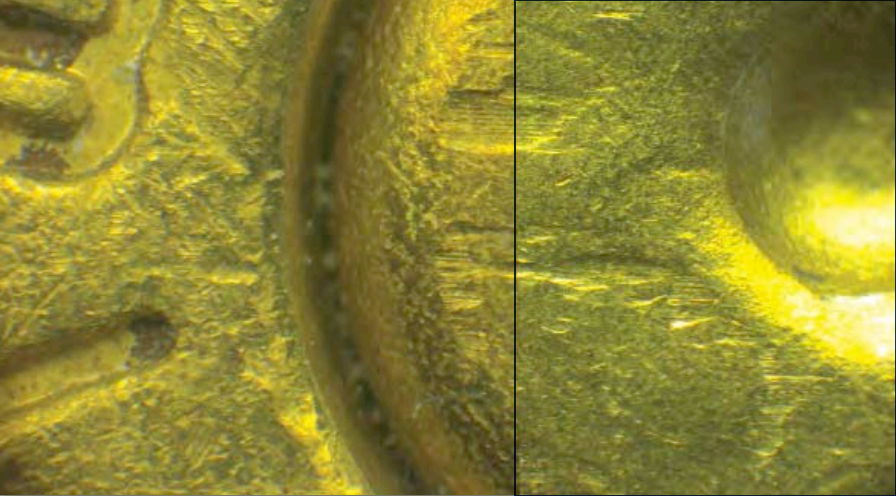
\includegraphics[width=\textwidth]{images/cartridgeCasePair_comparison_with_line} \caption{\label{fig:ccPair_combined} A cartridge case pair with visible breech face impressions under a microscrope.  A thin line can be seen separating the two views. The degree to which the markings coincide is used to conclude whether the pair comes from the same source.}\label{fig:unnamed-chunk-3}
\end{figure}
\end{Schunk}

\autoref{fig:ccPair_combined} is an example of an image from a
comparison microscope used by firearms examiners in laboratory settings.
Digital microscopy is capable of precision measurements of surface
topology at even higher resolutions. Using a 3D microscope, we can
obtain scans of breech face impressions at the micron level
(\(1 \mu m = 10^{-3} mm = 10^{-6} m\)). These 3D topological scans are
used as input to automated comparison algorithms, such as the CMC method
originally proposed in \citet{song_proposed_2013}.

\hypertarget{cmcMethod}{%
\section{The CMC method}\label{cmcMethod}}

In this section, we examine the process of implementing the CMC method
for automatic comparisons of 3D cartridge case scans. At each step, we
will compare the description in the published papers with the
implementation in code, discussing the gaps in the method description
and how we filled in those gaps during the creation of \CRANpkg{cmcR}.

All of the CMC methods can be broken down into three broad stages: (1)
preprocessing, (2) cell-based similarity feature extraction, and (3)
application of a decision rule as illustrated in
\autoref{fig:overview-flow}. In the following sections we break each of
these stages further into a set of modular steps. One advantage of
modularizing these algorithms is that we can implement an algorithm as a
set of sequential procedures. This allows us to test new variations
against the old implementation in a coherent, unified framework.

\begin{figure}
\centering
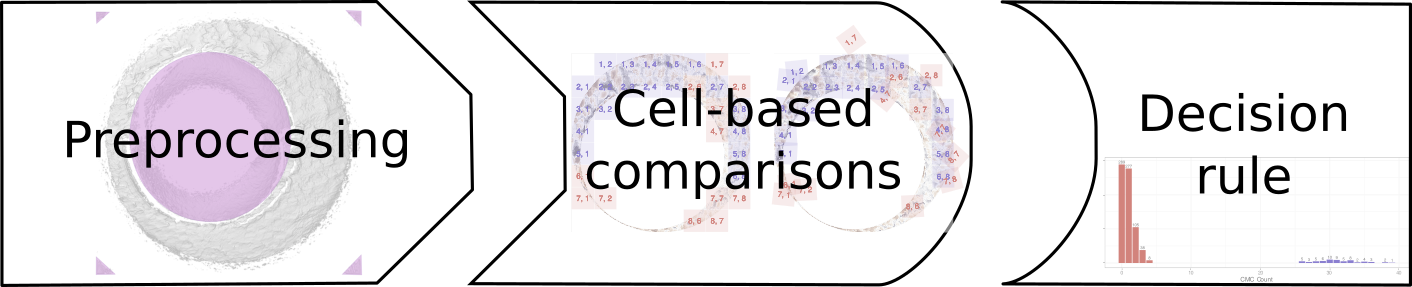
\includegraphics[width=.8\textwidth]{images/overview-flow.png}
\caption{The stages of CMC methods. In the preprocessing stage, each scan is prepared for analysis, removing extraneous information and noise. Then, each scan is broken up into cells, which are numerically compared to cells in the other scan to determine an optimal alignment. Finally, each of the scores arising from the cells in the second stage are compared to a reference distribution to determine whether the scans originate from the same source or from different sources.\label{fig:overview-flow}}
\end{figure}

The primary difference between the original and High CMC methods lies in
how the decision rules are utilized to separate matches and non-matches.
Beyond that there are also several small differences in the
preprocessing and comparison procedures. Current CMC papers lack
justification for changing these procedures. At the same time, different
conditions have been shown to yield very different results; even when
applying the same decision rule. This sensitivity of various methods to
different conditions has also not been discussed appropriately.

In this section, we discuss each stage of the CMC method using excerpts
from the original papers. Then, we examine the implementation of each
sub-procedure in the \CRANpkg{cmcR} package, considering the differences
between the textual description and its algorithmic translation.

\hypertarget{initialData}{%
\subsection{Initial Data}\label{initialData}}

Cartridge case scans are commonly stored in the ISO standard x3p file
format \citep{ISO25178-72}. x3p is a container format which consists of
a single surface matrix representing the height value of the breech face
surface and metadata concerning the parameters under which the scan was
taken (size, resolution, creator, microscope, and microscopy software
versions etc.). The \CRANpkg{x3ptools} package \citep{x3ptools} provides
functionality to work with the format in R.

\autoref{fig:cartridgeCasePair} shows the surface matrices of a known
match (KM) pair of cartridge cases from a study by
\citet{fadul_empirical_2011}. In this study, a total of 40 cartridge
cases were scanned with a lateral resolution of 6.25 microns
(micrometers) per pixel. The surface matrices are approximately
\(1200 \times 1200\) pixels in size corresponding to an area of about
\(3.8 \times 3.8\) mm\(^2\).

\begin{Schunk}
\begin{figure}[htbp]

{\centering \subfloat[\label{fig:rawBFs-1}]{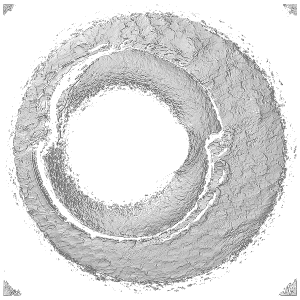
\includegraphics[width=.49\linewidth,height=.49\linewidth]{derivatives/fadul1-1} }\subfloat[\label{fig:rawBFs-2}]{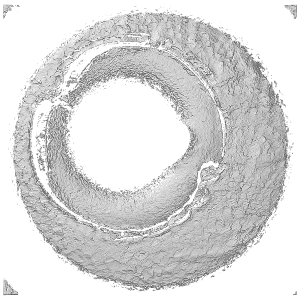
\includegraphics[width=.49\linewidth,height=.49\linewidth]{derivatives/fadul1-2} }

}

\caption{\label{fig:cartridgeCasePair} Unprocessed surface matrices of the known-match Fadul 1-1 (left) and Fadul 1-2 (right) \citep{fadul_empirical_2011}. The observations in the corners of these surface matrices are artifacts of the staging area in which these scans were taken. The holes on the interior of the primer surfaces are caused by the firing pin striking the primer during the firing process. The region of the primer around this hole does not come into uniform contact with the breech face of the firearm.}\label{fig:rawBFs}
\end{figure}
\end{Schunk}

Only certain regions of a cartridge case contain identifying breech face
impression markings. \citet{song_proposed_2013} defines ``valid
correlation regions'' as regions where ``the individual characteristics
of the ballistics signature are found that can be used effectively for
ballistics identification.'' Prior to applying the CMC comparison
procedure, cartridge scans must undergo some preprocessing to identify
these valid correlation regions.

\hypertarget{preProcessing}{%
\subsection{Preprocessing procedures}\label{preProcessing}}

During the preprocessing stage, a series of sequential steps is used to
prepare each cartridge case for analysis. The goal of this process is to
remove the edges and center of the scan which did not come into contact
with the breech face, as well as any artifacts of the scan and
microscope staging which do not accurately represent the breech face
surface.

The different iterations of the CMC algorithm describe different
variations of these steps. A summary of these steps is shown in
\autoref{fig:preprocessing-schematic}.

\begin{figure}
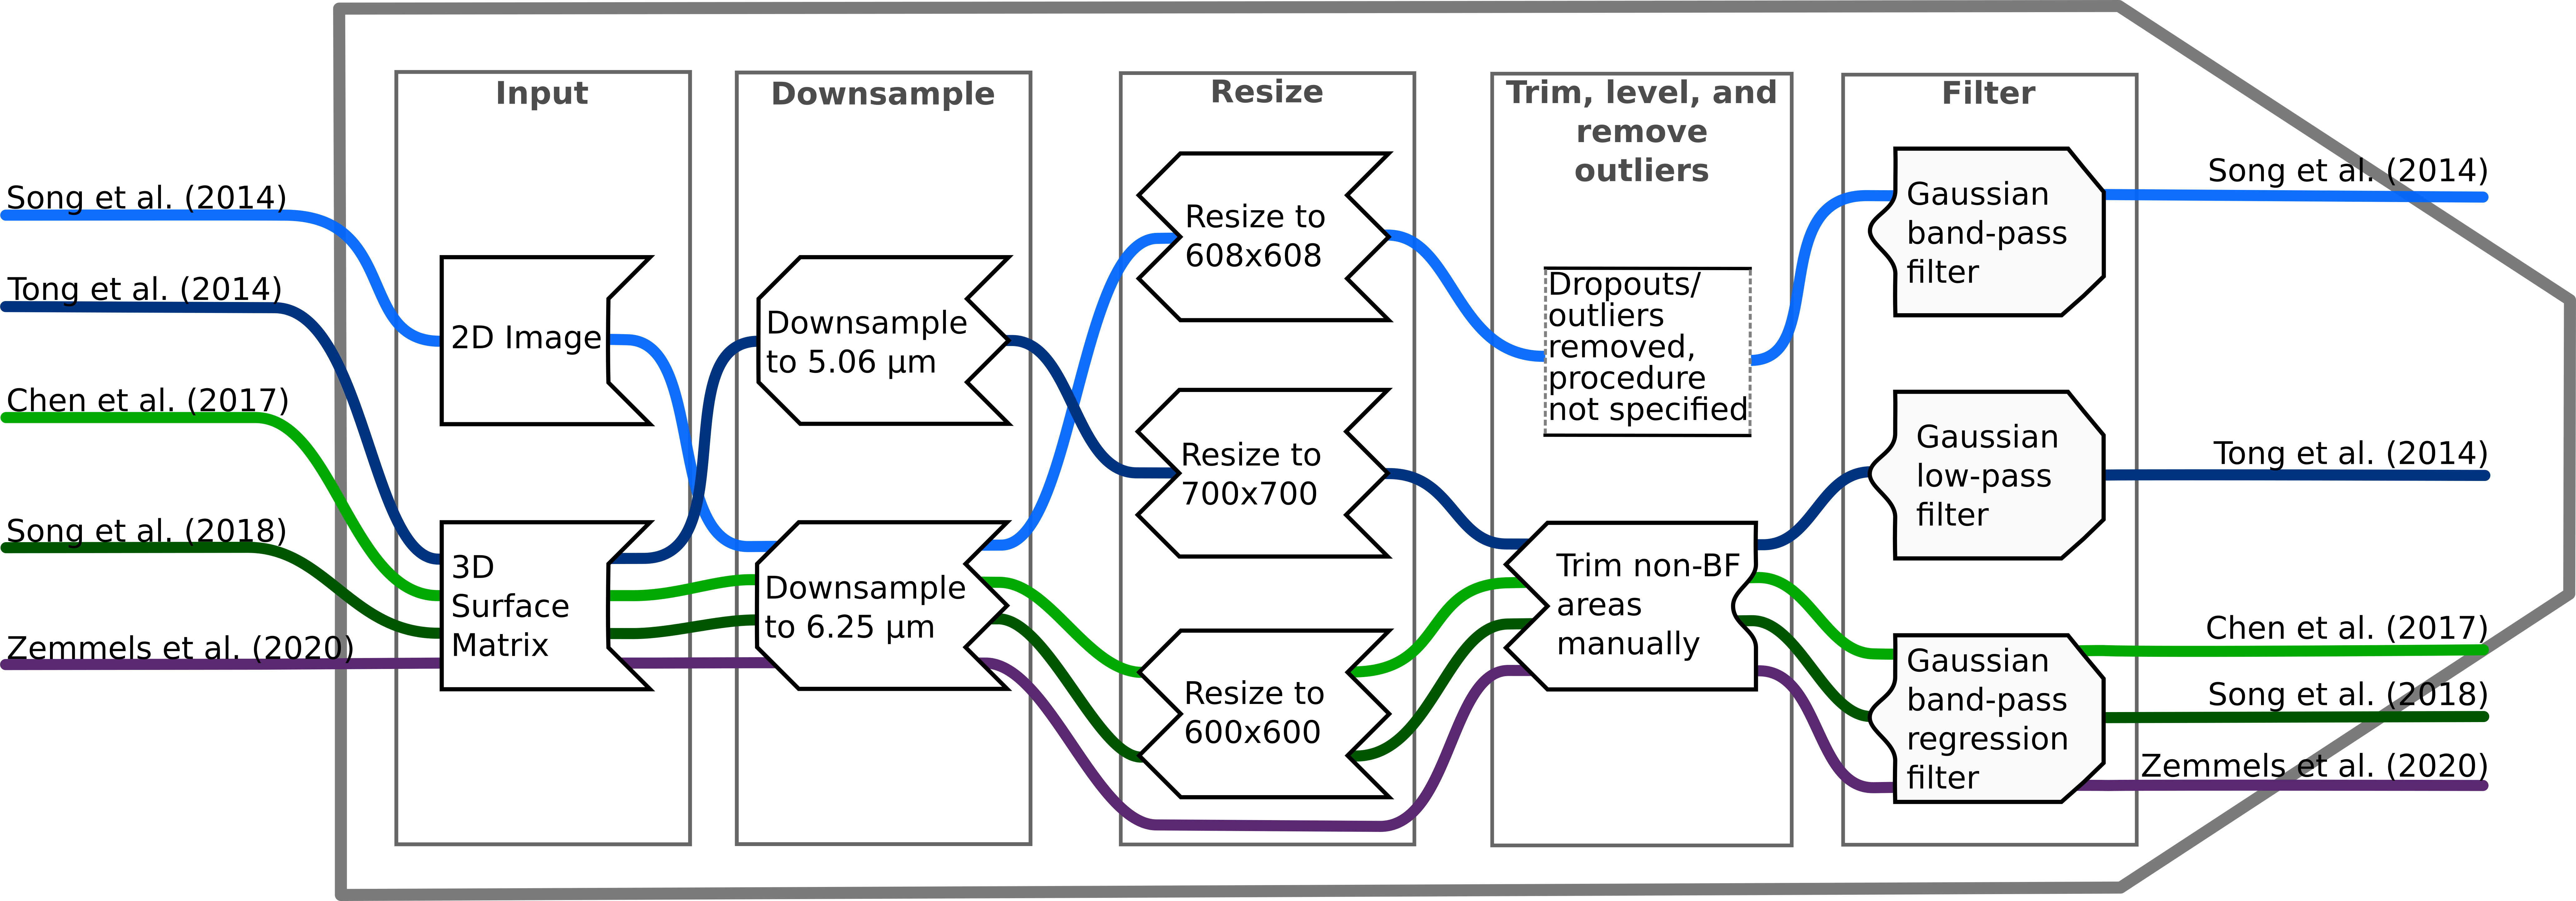
\includegraphics[width=\linewidth]{images/preprocessing_flow.png}
\caption{Overview of the set of pre-processing steps used in the CMC algorithms. Where a procedure step is not discussed or explicitly not applied in the paper, the path traverses empty space.}\label{fig:preprocessing-schematic}
\end{figure}

The implementation in \citet{tong_fired_2014} describes the
preprocessing steps (for the 2D images) as:

\begin{quote}
After trimming processing {[}sic{]} to remove unrelated correlations
areas, the final image size is reduced to 700 × 700 pixel with an
estimated pixel spacing of 5.0 \(\mu\)m. A Gaussian smoothing filter
(standard deviation \(\sigma\) = 1) was implemented first to remove high
frequency noise.
\end{quote}

Complicating the issue of preprocessing the scans, the procedures used
to process the surface matrices differ in each of the papers discussed
here. \citet{song_3d_2014} outline the following preprocessing
procedure:

\begin{quote}
Trim off the inside firing pin surface and other areas outside the
breech face mark, so that only breech face impression data remain for
correlation.
\end{quote}

\begin{quote}
Identify and remove dropouts or outliers.
\end{quote}

\begin{quote}
Apply a band-pass Gaussian regression filter with 40 \(\mu\)m short
cutoff length and 400 \(\mu\)m long cutoff length to remove low
frequency components, including surface curvature, form error, waviness
and high frequency components which mainly arise from the instrument
noise.
\end{quote}

While not explicitly mentioned in \citet{song_3d_2014},
\citet{song_estimating_2018} indicates that the ``trimming'' of the
unwanted regions of the scan is performed manually. No further
information is given in the paper describing what criteria were used for
this process; nor are the trimmed scans provided as intermediate data
for the sake of reproducibility.

It is also unclear how the dropouts and outliers are ``removed'' from
the scan or even how outliers are defined; many different methods for
outlier detection and removal are used in surface metrology
\citep{outlierdetection}. Most of these algorithms require the user to
select thresholds or parameters; thus, without any details about how the
outlier detection process was implemented, this portion of
\citet{song_3d_2014} is not reproducible.

We are not aware of an open-source implementation of the multivariate
band-pass Gaussian regression filter used in surface metrology
\citep{ISO16610-71}. Further, there are various parameters requiring
specification to implement a Gaussian regression filter and it is not
clear how these parameters were chosen
\citep{brinkman_bodschwinna_2003}.

As a result of these ambiguities, during our implementation of the
preprocessing algorithm, we had to make several educated guesses in
order to match the described procedure (and reported results) as closely
as possible.

\hypertarget{implementation-of-preprocessing-procedures}{%
\subsubsection{Implementation of preprocessing
procedures}\label{implementation-of-preprocessing-procedures}}

The preprocessing procedures are implemented via modularized functions
of the form \code{preProcess\_*}. Modularizing the steps of the
preprocessing procedures makes the overall process easier to understand
and allows for experimentation. \autoref{fig:processingPipeline} shows
an overview of the preprocessing framework for the Fadul 1-1 breech face
from reading the scan (left) to an analysis-ready region (right)\}. For
each scan in \autoref{fig:processingPipeline}, eleven height value
percentiles: the Minimum (0th), 1st, 2.5th, 10th, 25th, Median (50th),
75th, 90th, 97.5th, 99th, and Maximum (100th) are mapped to a
purple-to-orange color gradient. This mapping is chosen to highlight the
extreme values in each scan.

\begin{Schunk}
\begin{figure}[htbp]

{\centering 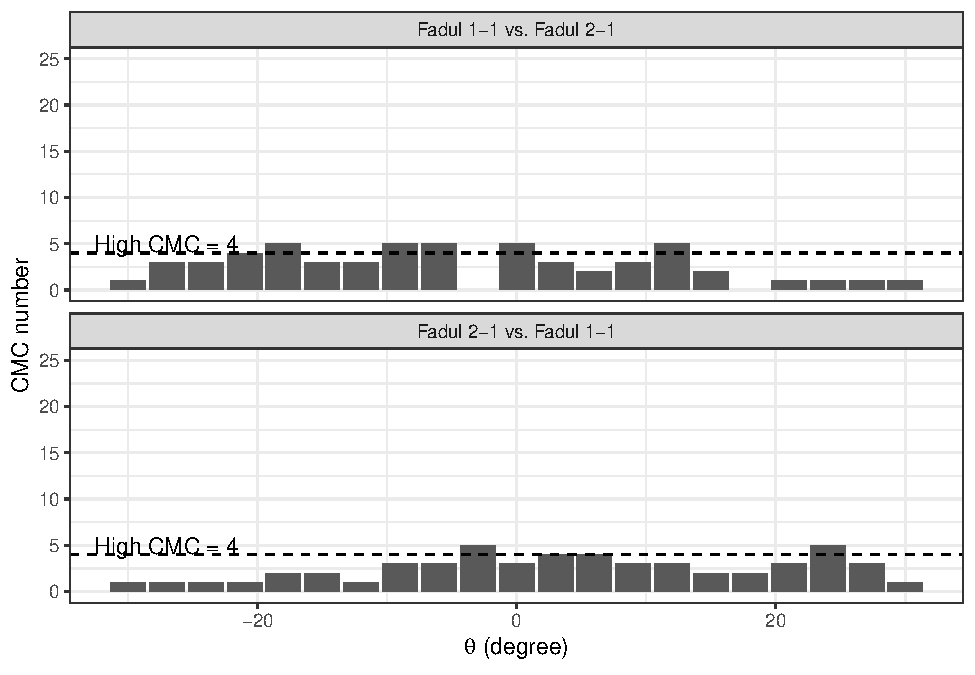
\includegraphics[width=\textwidth]{zemmels-vanderplas-hofmann_files/figure-latex/unnamed-chunk-5-1} 

}

\caption{\label{fig:processingPipeline} Illustration of the  preprocessing pipeline implemented in \CRANpkg{cmcR}.  At each stage, the variability in height across the scan decreases as extraneous sources of noise are removed.}\label{fig:unnamed-chunk-5}
\end{figure}
\end{Schunk}

We demonstrate usage of the \code{preProcess\_*} functions on the Fadul
1-1 scan. Each code chunk is followed up with an explanation of the
functions used.

\begin{Schunk}
\begin{Sinput}
# Step (1)
fadul1.1 <- x3ptools::x3p_read("data/fadul1-1.x3p")
\end{Sinput}
\end{Schunk}

We begin with a 3D scan. Typically, scans are downsampled to about 25\%
of their size by only retaining every other row and column in the
surface matrix. The breech faces in \citet{fadul_empirical_2011} were
initially scanned at a resolution of 3.125 \(\mu\)m per pixel.
Downsampling reduces the resolution to 6.25 \(\mu\)m per pixel. Step (1)
in \autoref{fig:processingPipeline} shows an unprocessed breech face
scan.

\begin{Schunk}
\begin{Sinput}
# Step (2)
fadul1.1_cropped <- fadul1.1 %>%
  cmcR::preProcess_crop(region = "exterior") %>%
  cmcR::preProcess_crop(region = "interior")
\end{Sinput}
\end{Schunk}

Three major regions of the scan are identified via a labeling algorithm
as described in \citet{hesselink_concurrent_2001} and available in the
\CRANpkg{imager} package \citep{imager}. These regions are the circle
capturing the exterior of the cartridge case primer, the breech face
impression region, and the circle around the firing pin impression hole
in the center of the scan.

The goal is to isolate the breech face impression region by removing
(i.e., replacing with \code{NA}) the pixels in the other two regions.
Upon labeling the different regions of the cartridge case scan, the
centers and radii of the cartridge case primer and firing pin impression
hole are estimated. This estimation procedure may require some user
input depending on how much of the exterior/interior the user wants
removed. The resulting breech face scan, like the one shown in step (2)
of \autoref{fig:processingPipeline}, is reproducible assuming the same
user-specified settings are used (if they are used at all). The
\code{preProcess\_crop} function removes the exterior and firing pin
impression region on the interior based on the \code{region} argument.

\begin{Schunk}
\begin{Sinput}
# Step (3)
fadul1.1_deTrended <- fadul1.1_cropped %>%
  preProcess_removeTrend(statistic = "quantile", tau = .5, method = "fn")
\end{Sinput}
\end{Schunk}

In step (3) any existing large-scale trend in the breech face scan
height values are removed. In steps (1) and (2) of
\autoref{fig:processingPipeline} it is clear that there is a
southwest-to-northeast trend in height values. Such a trend is
observable in many cartridge case scans, yet does not occur consistently
across cartridge cases fired from the same firearm. This indicates that
a trend in height values is likely to be an artifact of the scanning
process resulting from cartridge cases not being precisely, horizontally
leveled prior to taking the scan. Neglecting to remove these trends
leads to very different results based on our implementation. In an
extreme situation, two different-source cartridge cases with similar
trends might be incorrectly deemed ``congruent.'' The
\code{preProcess\_removeTrend} functions levels the breech face
impression regions obtained from step (2). The function estimates and
subtracts the conditional median via a quantile regression as
implemented in the \code{rq} function of the \CRANpkg{quantreg} package
\citep{quantreg}. Step (3) of \autoref{fig:processingPipeline} shows a
median-leveled breech face scan.

\begin{Schunk}
\begin{Sinput}
# Step (4)
fadul1.1_processed <- fadul1.1_deTrended %>%
  preProcess_gaussFilter(filtertype = "bp", wavelength = c(16,500)) %>%
  x3ptools::x3p_sample(m = 2)
\end{Sinput}
\end{Schunk}

In the final preprocessing step, a band-pass filter is applied to the
processed breech face scan to reduce the effects of undesired
frequencies in the comparison procedure. For example, low frequency
(large wavelength) global structure may exist in a cartridge case scan
due to manufacturing specifications. In forensics, this type of
structure is referred to as a class or subclass characteristic -- it is
shared by many objects of the same make and model. Class characteristics
are used by forensic practitioners to initially pare down the possible
pool of matching cartridge cases \citep{firearm_id_thompson}. While this
additional global structure may assist with matching cartridge cases, it
can also artificially inflate the probability of making a false-positive
identification. The goal of comparing breech-face scans is to answer the
question of source. Same-sourceness can only be determined by matching
individual characteristics, so the global structure is removed by using
a high-pass Gaussian filter. Similarly, a low-pass filter is used to
remove noise and outliers from cartridge case scans due to, for example,
imperfections in the scanning process. A band-pass Gaussian filter
combines the effects of low and high-pass filters; this is the default
choice in \CRANpkg{cmcR}. The band-pass filtered breech face scan as
returned by the \code{preProcess\_gaussFilter} function is shown in the
fourth panel of \autoref{fig:processingPipeline}.

There is currently no determination or removal of outliers in the
\CRANpkg{cmcR} package's preprocessing procedures. Instead, we rely on
the low-pass portion of the Gaussian filter to reduce the effects of any
high-frequency noise.

\autoref{fig:processedScans} displays the processed Fadul 1-1 and Fadul
1-2 scans; the second matrix is processed using the same parameters.
Similarity features are extracted from a processed cartridge case pair
in the cell-based comparison procedure.

\begin{Schunk}
\begin{figure}[htbp]

{\centering 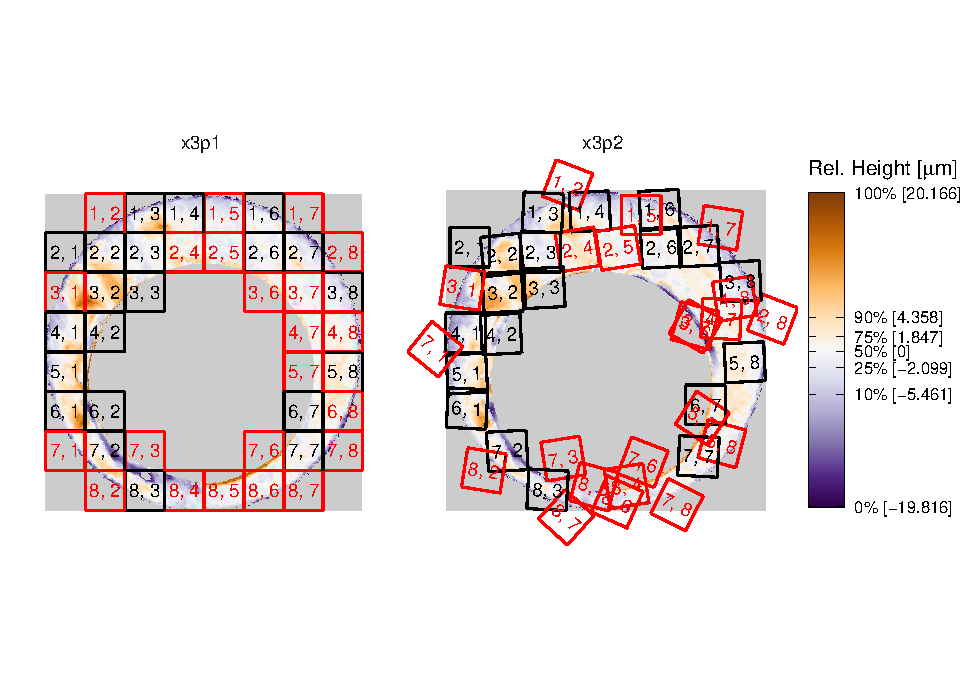
\includegraphics[width=\textwidth]{zemmels-vanderplas-hofmann_files/figure-latex/unnamed-chunk-10-1} 

}

\caption{\label{fig:processedScans} Fadul 1-1 and Fadul 1-2 after preprocessing. Similar striated markings are now easier to visually identify on both surfaces. It is now clearer that one of the scans needs to be rotated to align better with the other.}\label{fig:unnamed-chunk-10}
\end{figure}
\end{Schunk}

\hypertarget{comparisonProcedure}{%
\subsection{``Correlation cell'' comparison
procedure}\label{comparisonProcedure}}

As described in \citet{song_proposed_2013}, breech face markings are not
uniformly impressed upon a cartridge case during the firing process. As
such, only certain sections of the cartridge case are used in a
comparison. In the CMC method as proposed by \citet{song_proposed_2013}
two scans are compared by partitioning one breech face scan into a grid
of so-called ``correlation cells''. These cells are compared
individually to their best-matching counterpart on the other scan. If a
large proportion of these correlation cells are highly similar to their
counterparts on the other breech face scan, this is considered as
evidence that the markings on the two cartridge cases were made by the
same source. The number of highly similar cells is defined as the
\dfn{CMC count} \(C\) \citep{song_proposed_2013} of the breech-face
comparison. The CMC count is considered to be a more robust similarity
metric than a cross-correlation score based on the entire cartridge
case.

\begin{Schunk}
\begin{figure}[htbp]

{\centering 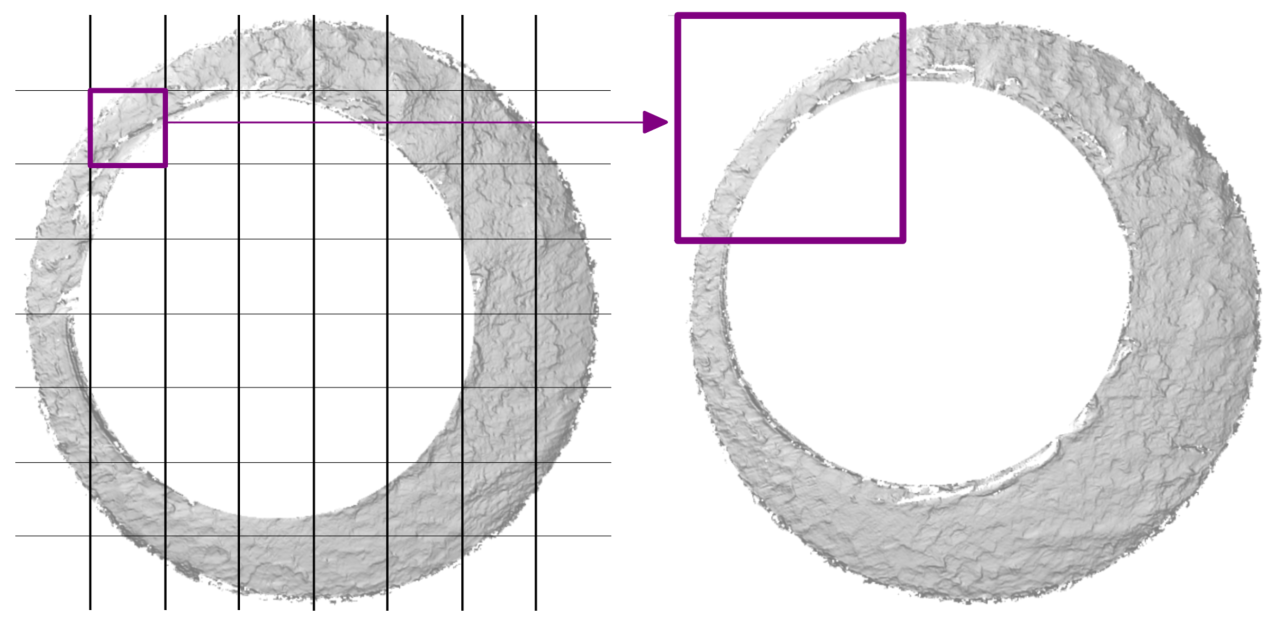
\includegraphics[width=.75\textwidth]{images/cmc_illustration} 

}

\caption{\label{fig:cmc_illustration} Illustration of comparing a cell in the reference cartridge case scan (left) to a larger region in a questioned cartridge case scan (right). Every one of the cells in the reference cartridge case is similarly paired with a region in the questioned cartridge case.  To determine the rotation at which the two cartridge cases align, the cell-region pairs are compared for various rotations of the questioned cartridge case.}\label{fig:unnamed-chunk-11}
\end{figure}
\end{Schunk}

\autoref{fig:cmc_illustration} illustrates the cell-based comparison
procedure between two cartridge case scans. The scan on the left serves
as the reference; it is divided into a grid of \(k \times k\) cells. The
cell size (and thus, the corresponding number of cells) is optimized
experimentally:

\begin{quote}
The cell size must be experimentally optimized, not too small and not
too large. Either condition may result in low correlation accuracy. For
the initial tests of 9 mm caliber cartridge cases, good correlation
results for breech face correlations were obtained using the cell sizes
ranging from (0.25 × 0.25) to (0.5 × 0.5) \(mm^2\). \citep{song_3d_2014}
\end{quote}

\begin{figure}
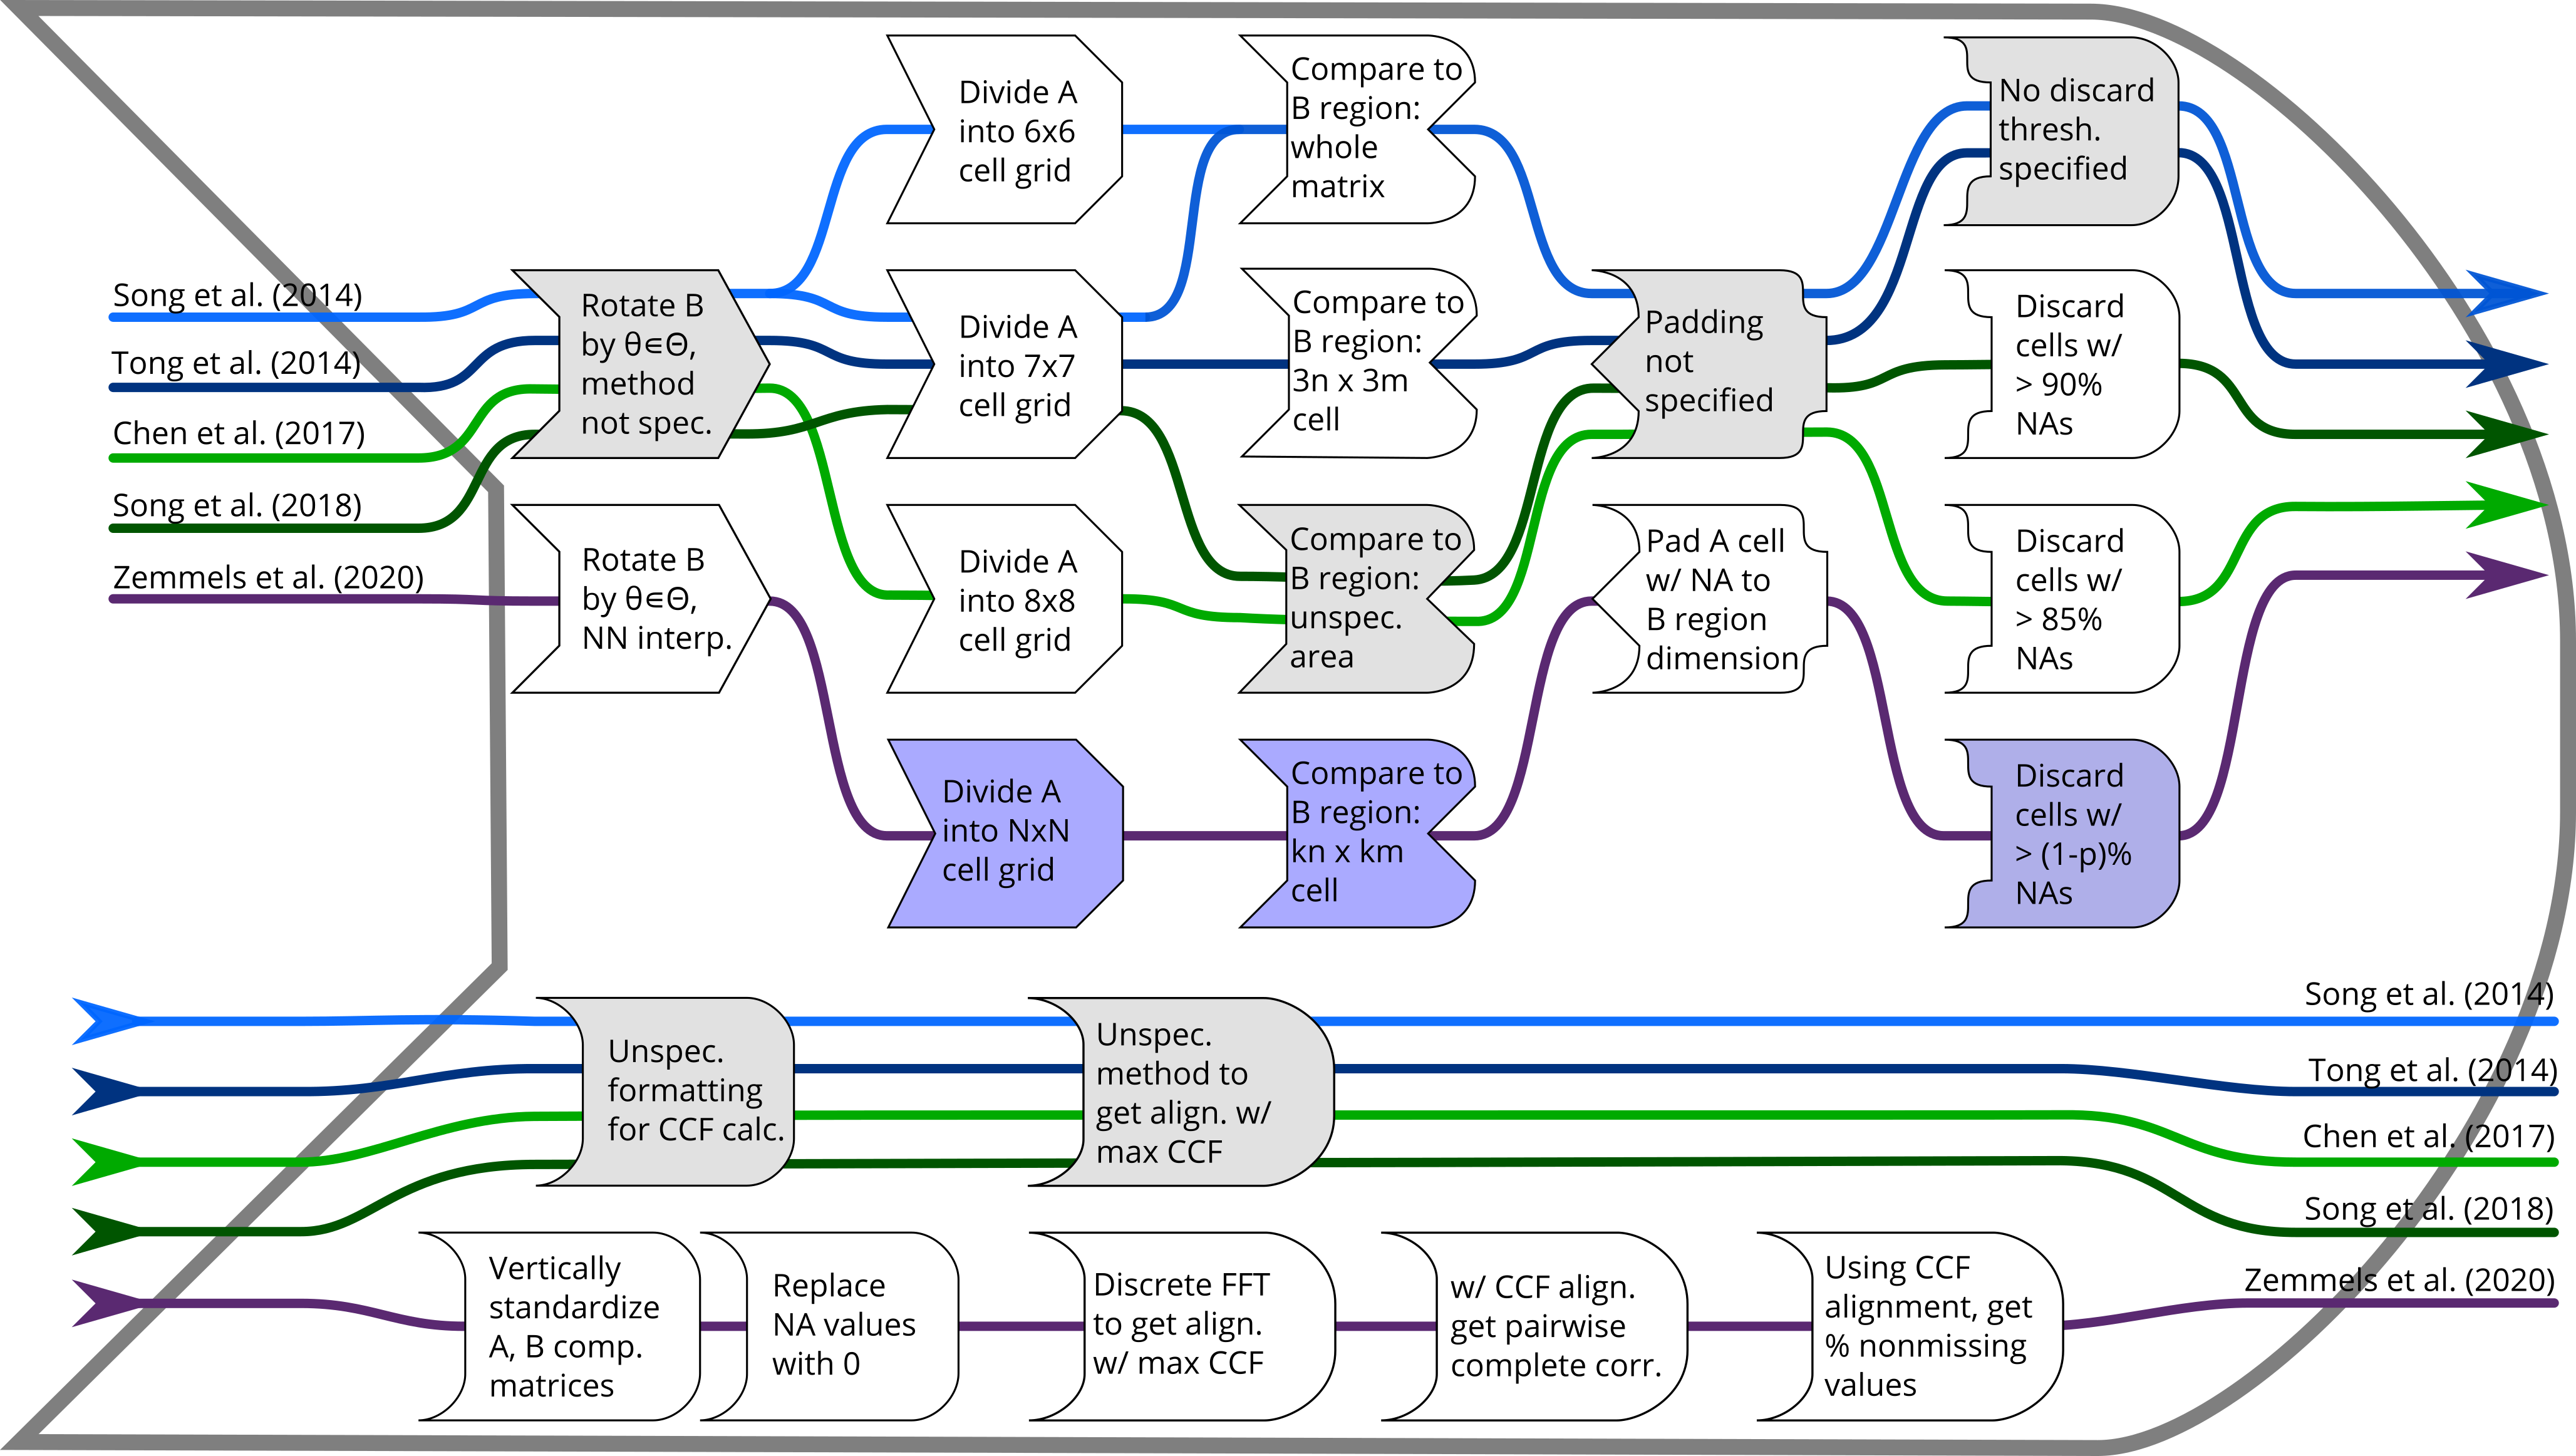
\includegraphics[width=\textwidth]{images/cmc_flow.png}
\caption{Each CMC implementation uses a slightly different procedure to obtain a similarity score between two cartridge cases. Steps which are implemented with additional user-specified parameters are shaded purple; steps which are described but without sufficient detail are shaded grey.}\label{fig:cmc-schematic}
\end{figure}

\autoref{fig:cmc-schematic} shows the steps of the correlation cell
comparison process in each of the papers as well as the \CRANpkg{cmcR}
implementation. Each cell is paired with an associated larger region in
the other scan. The absolute location of each cell and region in their
respective surface matrices remain constant. However, the scan on the
right is rotated to determine the rotation at which the two scans are
the most ``similar,'' as quantified by the
\dfn{cross-correlation function} (CCF).

For a real-valued matrices \(A\) and \(B\) of dimension \(M \times N\)
and \(P \times Q\), respectively, the cross-correlation function,
denoted \((A \star B)\) is defined as \[
(A \star B)[m,n] = \sum_{i=1}^M \sum_{j=1}^N A[i,j] B[(i + m), (j + n)],
\] where \(-(P-1) \leq m \leq M-1\) and \(-(Q-1) \leq n \leq N-1\). By
this definition, the \([m,n]\)th element of the resulting
\(M + P - 1 \times N + Q - 1\) CCF matrix quantifies the similarity
between matrices \(A\) and \(B\) for a translation of matrix \(B\) by
\(m\) pixels horizontally and \(n\) pixel vertically. The index at which
the CCF attains a maximum represents the optimal translation needed to
align \(B\) with \(A\). The CCF as defined need not be bounded between
\(-1\) and \(1\). However, it is common to normalize the CCF for
interpretability, and this is the convention adopted by the
\CRANpkg{cmcR} package.

Prior to calculating the CCF, the matrices \(A\) and \(B\) are
standardized through subtraction of their respective means and division
by their respective standard deviations. This is referred to as the
\dfn{Areal Cross-Correlation Function} (ACCF) in some CMC papers
\citep{ott_applying_2017}. A direct calculation of the CCF for breech
face scans based on the definition above is inhibitingly slow. While
computationally feasible alternatives exist, \citet{song_proposed_2013}
and other CMC papers do not specify the algorithm used to calculate the
CCF.

In \citet{song_3d_2014}, the comparison process is described with
characteristic brevity:

\begin{quote}
CMC pairs are identified by three types of identification parameters:
the correlation value CCF\(_{\max}\), registration angle \(\theta\) and
translation distances \(x\), \(y\) with thresholds \(T_{\text{CCF}}\),
\(T_\theta\) and \(T_x, T_y\), respectively. The correlated cell pairs
are considered as CMCs when their correlation value CCF\(_{\max}\),
\(T_{\text{CCF}}\), and their registration angle \(\theta\) and \(x-y\)
registration pattern are within the thresholds \(T_\theta\), and
\(T_x, T_y\).
\end{quote}

Note, that rotating an image or breech face scan by an arbitrary angle
(other than a multiple of 90 degrees) requires interpolating new pixel
locations. A variety of interpolation schemes exist
\citep{parker_comparison_1983}, but there are no details provided in the
papers under consideration indicating which interpolation algorithm was
used. In \CRANpkg{cmcR}, surfaces matrices are rotated using a
``nearest-neighbor'' interpolation scheme \citep{imager}.

In the next section, we discuss our implementation of the cell-based
comparison procedure.

\hypertarget{implementation-of-the-correlation-cell-comparison-procedure}{%
\subsubsection{Implementation of the correlation cell comparison
procedure}\label{implementation-of-the-correlation-cell-comparison-procedure}}

All of the steps dealing with cell-based comparisons are implemented as
functions of the form \code{comparison\_*}. Similar to the
\code{preProcess\_*} functions, the \code{comparison\_*} functions can
be chained together through a sequence of pipes.

Published implementations of the CMC algorithm do not describe precisely
how the CCF is calculated. In image processing, it is common to use an
implementation based on the Fast Fourier Transform
\citep{Brown92asurvey}. This implementation leverages the
Cross-Correlation Theorem, which states that for matrices \(A\) and
\(B\), the CCF can be expressed in terms of frequency-domain pointwise
product: \[
(A \star B )[m,n]= \mathcal{F}^{-1}\left(\overline{\mathcal{F}(A)} \odot \mathcal{F}(B)\right)[m,n]
\] where \(\mathcal{F}\) and \(\mathcal{F}^{-1}\) denote the discrete
Fourier and inverse discrete Fourier transforms, respectively, and
\(\overline{\mathcal{F}(A)}\) denotes the complex conjugate
\citep{fft_brigham}. Because the product on the right-hand side is
calculated pointwise, this result allows us to trade the moving sum
computations from the definition of the CCF for two forward Fourier
transformation, a pointwise product, and an inverse Fourier
transformation. The Fast Fourier Transform (FFT) algorithm can be used
to reduce the computational load considerably.

No computational shortcut comes without some tradeoffs, though, and this
FFT-based CCF calculation is no different. The FFT does not tolerate
missing values, and breech faces are not continuous surfaces -- all of
the white regions in \autoref{fig:cmc_illustration} correspond to
missing values. While it is unclear how the CCF is implemented in the
CMC papers (it is not even defined mathematically), the \CRANpkg{cmcR}
package adopts the following conventions:

\begin{itemize}
\item
  Only cells with a minimum proportion of non-missing pixels are
  assessed. This minimum threshold differs across CMC papers (15\% in
  \citet{chen_convergence_2017} vs.~10\% in
  \citet{song_estimating_2018}, as shown in
  \autoref{fig:cmc-schematic}), and is referenced but not specified in
  several other papers
  \citep{tong_fired_2014,song_3d_2014,chu_validation_2013}. The
  \code{comparison\_calcPropMissing} function computes the proportion of
  a matrix that is missing (\code{NA}-valued).
\item
  Missing values are replaced with the overall mean value when the
  FFT-based CCF is computed (using function
  \code{comparison\_replaceMissing}).
\item
  The optimal translation is determined using the FFT-based CCF (using
  \code{comparison\_fft\_ccf}).
\item
  Based on the optimal translation determined from the FFT-based CCF, we
  compute the pairwise complete CCF directly, avoiding any distortion of
  the CCF computation based on compensation for missing values (using
  function \code{comparison\_cor}).
\end{itemize}

The code below demonstrates how the \code{comparison\_allTogether}
function can be used to perform the entire cell-based comparison
procedure in one call. The comparison procedure is performed twice: once
with Fadul 1-1 considered the ``reference'' scan divided into cells that
are compared to the ``target'' scan Fadul 1-2 and again with the roles
reversed.

\begin{Schunk}
\begin{Sinput}
# Fill in most of the arguments first
comp_w_pars <- purrr::partial(.f = comparison_allTogether, 
                               numCells = 64, maxMissingProp = .85)

# Then, map the remaining values to theta
kmComparisonFeatures <- purrr::map_dfr(
  seq(-30,30,by = 3), 
  ~comp_w_pars(reference = fadul1.1, target = fadul1.2, theta = .))

kmComparisonFeatures_rev <- purrr::map_dfr(
  seq(-30,30,by = 3), 
  ~comp_w_pars(reference = fadul1.2, target = fadul1.1, theta = .))
\end{Sinput}
\end{Schunk}

The \code{comparison\_allTogether} function consists of the following
steps wrapped into a single convenience function:

\begin{itemize}
\tightlist
\item
  \code{comparison\_cellDivision}: Divide the reference scan into cells
\item
  \code{comparison\_getTargetRegions}: Extract regions associated with
  each reference cell from the target scan
\item
  \code{comparison\_calcPropMissing}: Compute missing proportions and
  filter out cells with a proportion of missing values above the
  threshold.
\item
  \code{comparison\_standardizeHeights}: Standardize height values
\item
  \code{comparison\_replaceMissing}: Replace missing values
\item
  \code{comparison\_fft\_ccf}: Compute CCF and estimated translations
  using FFT
\item
  \code{comparison\_cor}: Compute pairwise-complete correlation between
  a reference cell and a matrix of the same size extracted from the
  associated target region
\end{itemize}

This sequence of functions are applied for a sequence of angles
\(\theta\) rotating the target scan relative to the reference scan. When
implementing the High CMC method \citep{tong_improved_2015}, both
combinations of reference and target scan are examined (e.g.~A-B and
B-A).

\autoref{tab:cellCCF} shows several rows of the data frame output of the
\code{comparison\_allTogether} function for the comparison of Fadul 1-1
vs.~Fadul 1-2 considering Fadul 1-1 as the reference scan. Although a
grid of \(8 \times 8\) cells was used, there were only 26 cell-region
pairs that contained a sufficient proportion of non-missing values (15\%
in this example). The features derived from the correlation cell
procedure (CCF\(_{max}\), \(\Delta x\), \(\Delta y\), \(\theta\)) are
used as inputs to the methods for assessing the similarity between
scans.

\begin{Schunk}
\begin{table}

\caption{\label{tab:unnamed-chunk-13}\label{tab:cellCCF} Example of output from correlation cell comparison procedure between Fadul 1-1 and Fadul 1-2 rotated by -24 degrees. Due to the large proportion of missing values that are replaced to compute the FFT-based correlation, the pairwise-complete correlation is most often greater than the FFT-based correlation.}
\centering
\begin{tabular}[t]{|cccrrr|}
\toprule
Cell Index & Pairwise-comp. corr. & FFT-based corr. & $\Delta$x & $\Delta$y & $\theta$\\
\midrule
\cellcolor{lightgray}{1, 2} & \cellcolor{lightgray}{0.630} & \cellcolor{lightgray}{0.214} & \cellcolor{lightgray}{31} & \cellcolor{lightgray}{22} & \cellcolor{lightgray}{-24}\\
1, 3 & 0.673 & 0.295 & -1 & 11 & -24\\
\cellcolor{lightgray}{1, 4} & \cellcolor{lightgray}{0.634} & \cellcolor{lightgray}{0.255} & \cellcolor{lightgray}{-2} & \cellcolor{lightgray}{7} & \cellcolor{lightgray}{-24}\\
1, 5 & 0.525 & 0.248 & -2 & 7 & -24\\
\cellcolor{lightgray}{1, 6} & \cellcolor{lightgray}{0.658} & \cellcolor{lightgray}{0.294} & \cellcolor{lightgray}{-1} & \cellcolor{lightgray}{7} & \cellcolor{lightgray}{-24}\\
\bottomrule
\end{tabular}
\end{table}

\end{Schunk}

\hypertarget{decision-rule}{%
\subsection{Decision Rule}\label{decision-rule}}

For each cell on the reference scan, a set of rotation angles \(\theta\)
with associated translations \((\Delta x, \Delta y)\) and
cross-correlation values are calculated. These sets need to be
aggregated into a single consensus decision. Here, we describe the two
methods implemented in the \CRANpkg{cmcR} package: the original decision
rule described in \citet{song_3d_2014} and the High CMC method proposed
in \citep{tong_improved_2015}.

The idea of a consensus decision is based on the assumption that a
matching pair of cartridge cases will have similar translation and
rotation values for all of the cells, while a non-matching pair of
cartridge cases will exhibit a variety of different translation and
rotation values without showing a particular pattern.

The first step in any CMC decision process is therefore to obtain a
consensus estimate of \(x, y, \theta\). Where the various CMC decision
rules principally differ is in how they identify a ``consensus'' among
the estimated \(x,y, \theta\) values.

\hypertarget{originalMethod}{%
\subsubsection{The Original CMC Method}\label{originalMethod}}

This section briefly describes the decision rule used in the first CMC
paper \citep{song_proposed_2013}. For a thorough explanation of the
procedure, refer to the
\href{https://csafe-isu.github.io/cmcR/articles/decisionRuleDescription.html}{CMC
Decision Rule Description} vignette in the \CRANpkg{cmcR} package.

Let \(x_i, y_i, \theta_i\) denote the translation and rotation
parameters which produce the highest CCF for the alignment of
cell-region pair \(i\), \(i = 1,...,n\) where \(n\) is the total number
of cell-region pairs containing a sufficient proportion of non-missing
values.

\citet{song_proposed_2013} propose the median as a consensus
\((x_{\text{ref}}, y_{\text{ref}}, \theta_{\text{ref}})\) across the
cell-region pairs for a particular cartridge case pair comparison. Then,
the distances between the consensus values and the values for each cell
comparison are assessed to determine whether the values are within a
specified distance of the consensus, as determined by three threshold
parameters \(T_{x}, T_{y}, T_\theta, T_{\text{CCF}}\).

A cell-region pair \(i\) is declared a match if all of the following
conditions hold:

\begin{eqnarray}\label{eq:original}
|x_i - x_{\text{ref}}| &\leq& T_{x} \\ \nonumber
|y_i - y_{\text{ref}}| &\leq& T_{y} \\ \nonumber
|\theta_i - \theta_{\text{ref}}| &\leq& T_{\theta} \\ \nonumber
\text{CCF}_{\max,i} &\geq& T_{\text{CCF}}.
\end{eqnarray}

The CMC count is then defined as the number of matching cell-region
pairs (out of \(n\)).

\citet{song_3d_2014} indicate that these thresholds need to be
determined experimentally. There is little consensus on an optimal set
of thresholds and no discussion of the sensitivity of proposed methods
to different threshold choices across CMC papers. As such, there is
little known about the effectiveness of the any CMC method to
``out-of-bag'' samples.

\autoref{tab:thresholdTable} summarizes the thresholds used in various
CMC papers.

\begin{table}[ht]
    \centering
    \begin{tabular}{|lrrr|}
      \hline
        Paper & Translation $T_x, T_y$ & Rotation $\theta$ & CCF$_{\max}$ \\
              & (in pixels) & (in degrees) \\
        \hline
        \cellcolor{lightgray}{\citet{song_3d_2014}} & \cellcolor{lightgray}{20} & 
        \cellcolor{lightgray}{6} & \cellcolor{lightgray}{.60} \\
        
        \citet{tong_fired_2014} & 30 & 3 & .25 \\
        
        \cellcolor{lightgray}{\citet{tong_improved_2015}} & \cellcolor{lightgray}{15} & 
        \cellcolor{lightgray}{3} & \cellcolor{lightgray}{.55} \\
        
        \citet{chen_convergence_2017} & 20 & 3 & .40 \\
        
        \cellcolor{lightgray}{\citet{song_estimating_2018}} & \cellcolor{lightgray}{20} & 
        \cellcolor{lightgray}{6} & \cellcolor{lightgray}{.50}\\
        \hline
    \end{tabular}
    \caption{Different thresholds for translation, rotation, and CCF$_{\max}$ are used across different papers. The range in CCF$_{\max}$ is particularly notable. There is currently no principled approach to determining these thresholds. Instead, thresholds seem to be chosen by authors through experimentation and selecting thresholds that provide promising results.}
    \label{tab:thresholdTable}
\end{table}

Unlike the original CMC method, the High CMC method considers multiple
rotations for each cell-region pair.

\hypertarget{highCMCMethod}{%
\subsubsection{The High CMC method}\label{highCMCMethod}}

For the High CMC method, comparisons between two scans are performed in
both directions, i.e.~each scan takes on the role of the reference scan
that is partitioned into a grid of cells. \citet{tong_improved_2015}
claim that in the original method, some matching cell-region pairs ``may
be mistakenly excluded from the CMC count'' because they attain the
largest CCF value at a rotation value outside the range allowed by
\(T_\theta\) ``by chance.''

To combat this, \citet{tong_improved_2015} introduce consensus values
across all cell-region pairs for each rotation angle \(\theta\) and
calcluate a \(\theta\) dependent CMC count as the sum of matches
observed. A match is defined, as previously if a cell-region pair \(i\)
fulfills the following three conditions:

\begin{eqnarray}\label{eqn:high-cmc}
|x_{i,\theta} - x_{ref,\theta}| &\leq& T_x \\ \nonumber
|y_{i,\theta} - y_{ref,\theta}| &\leq& T_y \\ \nonumber
\text{CCF}_{i,\theta} &\geq& T_{\text{CCF}}.
\end{eqnarray}

The \(\theta\)-dependent CMC count, CMC\(_\theta\), is then defined as
the sum of matching cell-region pairs.

\citet{tong_improved_2015} assert that for a truly matching cartridge
case pair, the relationship between \(\theta\) and CMC\(_\theta\) should
exhibit a ``prominent peak'' near the true rotation value at which the
pair aligns. In contrast, truly non-matching pairs should exhibit a
``relatively flat and random {[}\ldots{]} pattern.''

To determine whether a ``prominent peak'' exists in the relationship
between \(\theta\) and CMC\(_\theta\), \citet{tong_improved_2015}
introduce the ``angular range'' \(R (\tau)\) as an interval of rotation
angles covering high CMC\(_\theta\) values. Here, \(\tau\) represents
another threshold value that determines the angular range as the
interval of angles between
\(\arg \min_\theta CMC_\theta > CMC_{\text{max}} - \tau\) and and
\(\arg \max_\theta CMC_\theta < CMC_{\text{max}} - \tau\), where
\(CMC_{\text{max}}\) is defined as the maximum of CMC\(_\theta\) counts
across all rotation angles \(\theta\). \citet{tong_improved_2015}
suggest a value for \(\tau\) of 1 and further determine:

\begin{quote}
If the angular range of the ``high CMCs'' is within the range
\(T_\theta\), identify the CMCs for each rotation angle in this range
and combine them to give the number of CMCs for this comparison in place
of the original CMC number.
\end{quote}

If the angular range is outside the range of \(T_\theta\), we say that
the cartridge case pair ``fails'' the High CMC criteria and the original
CMC number is used. Using this definition, the High CMC method returns
for any comparison of breech face scans a CMC count equal to or higher
to the original method for both known matches and known non-matches.

\hypertarget{decisionRuleImplementation}{%
\subsubsection{Implementation of decision
rules}\label{decisionRuleImplementation}}

In this section, we demonstrate the implementation of the decision rules
in \CRANpkg{cmcR} for both the original method and the High CMC method.
For illustrative purposes, let us consider a particular set of
thresholds: \(T_x = T_y = 20\), \(T_{\theta} = 6\), and
\(T_{\text{CCF}} = .5\) values.

Decision rules in \CRANpkg{cmcR} are implemented as functions of the
form \code{decision\_*}. In particular, the \code{decision\_CMC}
function applies both the decision rule of the original method and the
High CMC method depending on whether a value for \(\tau\) is provided.
The code below demonstrates the use of \code{decision\_CMC} on the
features \code{kmComparisonFeatures}, extracted from the comparison of
scans Fadul 1-1 and Fadul 1-2. \code{kmComparisonFeatures\_rev} contains
the features from a comparison of Fadul 1-2 and Fadul 1-1. Addiionally,
we also compute the CMCs under both decision rules for the comparison
between the non-match pair Fadul 1-1 and Fadul 2-1 (not shown to avoid
redundancy).

\begin{Schunk}
\begin{Sinput}
kmComparison_cmcs <- kmComparisonFeatures %>% mutate(
  originalMethodClassif = 
    decision_CMC(cellIndex = cellIndex, x = x, y = y, theta = theta,
                 corr = pairwiseCompCor, xThresh = 20, thetaThresh = 6,
                 corrThresh = .5),
  highCMCClassif = 
    decision_CMC(cellIndex = cellIndex, x = x, y = y, theta = theta,
                 corr = pairwiseCompCor, xThresh = 20, thetaThresh = 6,
                 corrThresh = .5, tau = 1))
\end{Sinput}
\end{Schunk}

We can use the \code{cmcPlot} function to visualize CMCs and non-CMCs.
\autoref{fig:topVoteCMCPlot} shows congruent matching cells (CMCs) and
non-congruent matching cells (non-CMCs) determined under the original
method in blue and red, respectively. The (red) non-CMC patches are
located in the position where the maximum CCF value in the target scan
is attained. The top row shows 17 CMCs in blue and 10 non-CMCs in red
when Fadul 1-1 is treated as the reference and Fadul 1-2 the target. The
bottom row shows the 18 CMCs and 14 non-CMCs when the roles are
reversed. There is no discussion in \citet{song_proposed_2013} about
combining the results from these two comparison directions, but
\citet{tong_improved_2015} propose using the minimum of the two CMC
counts (17 in this example).

\begin{Schunk}
\begin{figure}[htbp]

{\centering 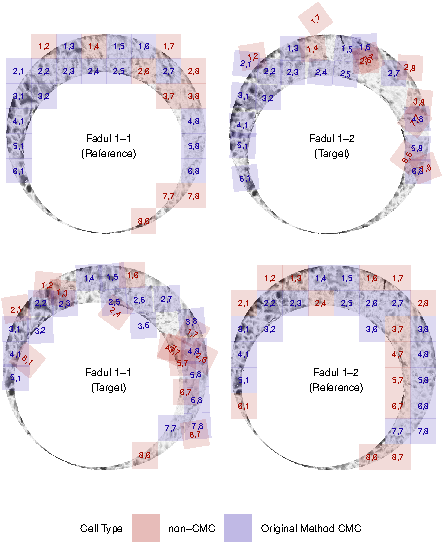
\includegraphics[width=\textwidth]{cmcR_files/figure-latex/kmOriginalMethod} 

}

\caption{\label{fig:topVoteCMCPlot} CMC results for the comparison between Fadul 1-1 and Fadul 1-2 using the original method. The two plots in the top row show the 17 CMCs when Fadul 1-1 is treated as the ``reference" cartridge case to which Fadul 1-2 (the ``target") is compared. The second row shows the 18 CMCs when the roles are reversed. Red cells indicate where cells \emph{not} identified as congruent achieve the maximum pairwise-complete correlation across all rotations of the target scan. }\label{fig:unnamed-chunk-16}
\end{figure}
\end{Schunk}

Similarly, CMCs and non-CMCs determined under the High CMC method are
shown in \autoref{fig:highCMCPlot}. Treating Fadul 1-1 and Fadul 1-2 as
the reference scan yields 19 and 18 CMCs, respectively. Combining the
results as described above, the final High CMC number is 24 CMCs.

\begin{Schunk}
\begin{figure}[htbp]

{\centering 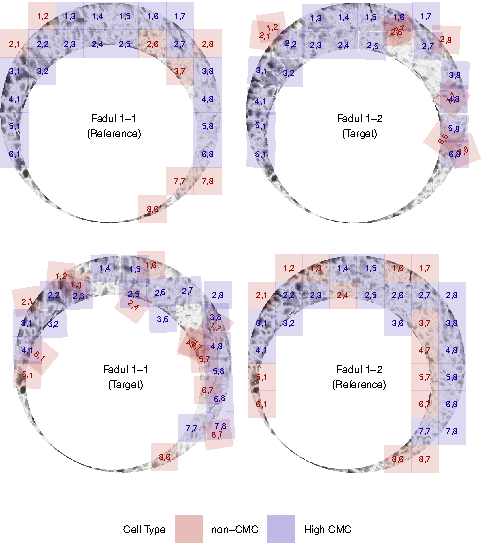
\includegraphics[width=\textwidth]{cmcR_files/figure-latex/kmHighCMC} 

}

\caption{\label{fig:highCMCPlot} Applying the High CMC method to the comparison of Fadul 1-1 and Fadul 1-2 results in 19 CMCs when Fadul 1-1 is treated as the reference (top) and 18 CMCs when Fadul 1-2 is treated as the reference (bottom). Although the individual comparisons do not yield considerably more CMCs than under the original CMC method, \citet{tong_improved_2015} indicate that the High CMCs from both comparisons are combined as the final High CMC count (each cell is counted at most once). Combining the results means that the High CMC method tends to produce higher CMC counts than the original CMC method. In this example, the combined High CMC count is 24 CMCs.}\label{fig:unnamed-chunk-17}
\end{figure}
\end{Schunk}

In contrast, \autoref{fig:knmCMCPlot} shows the CMC results for a
comparison between Fadul 1-1 and a known non-match scan, Fadul 2-1,
under the exact same processing conditions. Only one cell is classified
as a congruent matching cell under the original method when Fadul 1-1 is
the reference scan. No cells are classified as CMCs in the other
direction. While not shown, this pair fails the High CMC criteria and
thus was assigned 0 CMCs under the High CMC method.

\begin{Schunk}
\begin{figure}[htbp]

{\centering 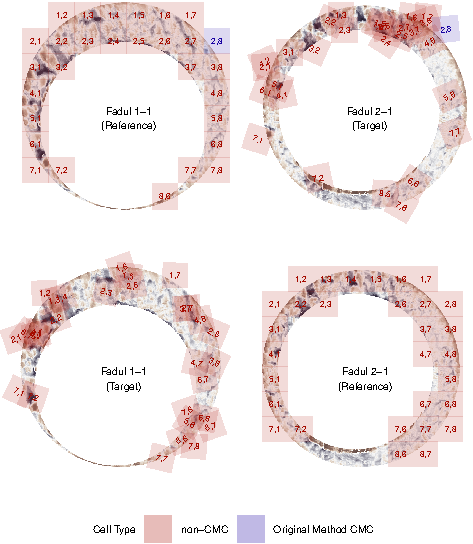
\includegraphics[width=\textwidth]{cmcR_files/figure-latex/knmOriginalMethod} 

}

\caption{\label{fig:knmCMCPlot} Applying both decision rules to the comparison between the non-match pair Fadul 1-1 and Fadul 2-1 results in 1 CMC under the original method (shown above) and 0 CMCs under the High CMC method (not shown). The seemingly random behavior of the red cells exemplifies the assumption that cells in a non-match comparison do not exhibit an observable pattern. Random chance should be the prevailing factor in classifying non-match cells as CMCs.}\label{fig:unnamed-chunk-18}
\end{figure}
\end{Schunk}

\hypertarget{ambiguities}{%
\subsection{Ambiguity in algorithmic descriptions}\label{ambiguities}}

During the implementation process we encountered various ambiguities in
the descriptions of the various CMC methods. In the following section we
investigate ways in which such ambiguities can be rectified by exploring
a set of reproducibility principles.

It is important to note that much of what we have presented as ``the CMC
method'' might not be considered as such by the original authors. In
particular, other authors might distinguish proposed methods based only
on how their decision rules differ. We include the preprocessing and
cell-based comparison procedures as part of the CMC methodology to
emphasize how much the final results depend on decisions made in these
first two steps. The preprocessing and cell-based comparison procedures
are discussed only briefly, if at all, in \citet{song_3d_2014},
\citet{tong_fired_2014}, \citet{tong_improved_2015}, or
\citet{chen_convergence_2017}, yet, the results reported often indicate
a sensitivity to these procedures. An actual sensitivity analysis of
proposed CMC methods has yet to be published. Left unchecked, this can
lead to results that are difficult to generalize to new data.

Apart from the CMC methods' generalizability, we also simply do not know
how the proposed methods are implemented. Ambiguities in the methods
range from minor implicit parameter choices (e.g., the convergence
criteria for the robust Gaussian regression filter
\citep{brinkman_bodschwinna_2003}) to procedures that fundamentally
change how similarity features are extracted and compared (e.g., how the
cross-correlation is calculated). As discussed in the
\protect\hyperlink{intro}{introduction}, this is an issue that pervades
computational research for which only verbal descriptions of algorithms
are provided. The only solution to such ambiguity is to enumerate,
implement, and pare-down the possible choices that could have been made
to arrive to published results. Unsurprisingly, this process takes a
considerable amount of time and resources that would be better spent
furthering the state of the field.

In the next section, we describe the process of resolving these
ambiguities in the CMC method descriptions. In doing so, we abstract a
set of principles by which methods and results can be rendered both
computationally reproducible and more thoroughly understood.

\hypertarget{investigation}{%
\section{Investigation of cell-based forensic pattern matching
methods}\label{investigation}}

As described in the \protect\hyperlink{initialData}{initial data}
section, the set of cartridge case scans from
\citet{fadul_empirical_2011} is commonly used to compare the performance
of various classification methods
\citep{song_3d_2014, tong_improved_2015, chen_convergence_2017}. This
set consists of 40 cartridge cases; 63 of which are known match pairs
and 717 known non-match pairs. Scans of each of the breech face
impression were taken with a Nanofocus Confocal Light Microscope at 10
fold magnification for a nominal lateral resolution of 3.125 microns per
pixel and published as part of NBTRD \citep{nbtrd}. While the exact
procedures by which these scans are processed are unavailable, these 3D
topographic surface images provide the basis of the comparison between
the implementation provided in the \CRANpkg{cmcR} package and published
results. However, justification for any differences will ultimately
involve educated hypothesization due to the closed-source nature of the
original implementations.

For any cartridge case pair, the number of CMCs can be determined under
the original method and the High CMC method described in
\protect\hyperlink{implementation}{implementation} section. We have
applied our implementation of these two methods to the 780 cartridge
case pairs available in the \citet{fadul_empirical_2011} data set under
a wide variety of processing conditions to determine which conditions
yield the best results while also matching the published results.
Perfect identification of all matching and non-matching pairs
corresponds to choosing a minimum CMC count threshold that separates the
distributions of the matching and non-matching CMC counts. A CMC count
threshold of 6 CMCs is generally accepted as the threshold in the
published papers {[}\citet{tong_improved_2015},
\citet{song_estimating_2018}, \citet{song_proposed_2013}{]}. However,
this threshold has been shown to not generalize well to all proposed
methods and cartridge case data sets \citep{chen_convergence_2017}. In
this section, we demonstrate that the ambiguities in the
\href{cmcMethod}{CMC method descriptions} and lack of guidance in the
choice of parameter settings propagate through the algorithm and produce
highly variable results. Additionally, wildly different parameter
settings are used by the same group of authors across different papers
as shown in \autoref{tab:thresholdTable}.

In the next section we focus on a discussion of the sensitivity of some
of the method's parameters. This presentation is far from exhaustive: we
primarily focus on the factors contributing to the most variable
results. As a consequence of this investigation we have developed a set
of principles designed to reduce the need for brute-force searches
across parameter settings when re-implementing algorithms without
accompanying code.

Adherence to these principles yields not only computationally
reproducible results, but also improves a reader's understanding of a
proposed method.

\hypertarget{communicating-a-methods-sensitivity-to-processing-conditions}{%
\subsection{Communicating a method's sensitivity to processing
conditions}\label{communicating-a-methods-sensitivity-to-processing-conditions}}

Choosing threshold values \(T_x, T_y, T_\theta, T_{\text{CCF}}\) for
translation, rotation and maximum cross-correlation is crucial in
declaring a particular cell-region pair ``congruent''. Many different
combinations of these thresholds yield perfect separation between the
matching and non-matching CMC count distributions. In situations where
ground truth is known, such as in the example of the Fadul data here, we
can use the ratio \(r\) of between- and within-group variability as an
additional statistic to measure separation between CMC counts of known
matches and known non-matches. Let C\(_{ij}\) denote the CMC count
assigned to the \(j\)th cartridge case pair, \(j = 1,...,n_i\),
\(n_1 = 63, n_2 = 717\), from the \(i\)th group, \(i = 1,2\)
representing matches and non-matches, respectively. For each set of
thresholds we calculate the \textbf{Variance Ratio} \(r\) as: \[
r = r\left(T_x, T_y, T_\theta, T_{\text{CCF}}\right) = \frac{\sum_{i=1}^2 \left(\overline{C}_{i.} - \overline{C}_{..}\right)^2}{\sum_{i=1}^2 \frac{1}{n_i - 1}\sum_{j=1}^{n_i} \left(C_{ij} - \overline{C}_{i.}\right)^2}
\] where \(\overline{C}_{i.}\) denotes the within-group CMC count
average and \(\overline{C}_{..}\) denotes the grand CMC count average.
Greater separation between and less variability within the match and
non-match CMC count distributions yields larger \(r\) values. Larger
values of \(r\) are therefore indicative of greater separation between
the groups.

\autoref{fig:decisionRuleSensitivity_comparison} shows results for the
original method and the High CMC method for a parameter setting of
\(T_{\Delta x} = 20 = T_{\Delta y}\) pixels, \(T_{\text{CCF}} = .5\),
and \(T_{\theta} = 6\). Both decision rules result in separated CMC
count distributions for known matches and known non-matches
corresponding to an AUC of 1.00. However, the High CMC decision rule
yields a larger separation between the known match and known non-match
distributions as evidenced by the considerably larger variance ratio
\(r\).

\begin{Schunk}
\begin{figure}[htbp]

\includegraphics[width=\textwidth]{zemmels-vanderplas-hofmann_files/figure-latex/unnamed-chunk-19-1} \hfill{}

\caption{\label{fig:decisionRuleSensitivity_comparison} CMC count relative frequencies under the original method and the High CMC method for $T_{\Delta x} = 20 = T_{\Delta y}$ pixels, $T_{\text{CCF}} = .5$, and $T_{\theta} = 6$ degrees. AUC $= 1.00$ corresponds to perfect separation of the match and non-match CMC count distributions. We can see that, for this set of processing parameters, the High CMC method yields higher CMC counts for known matches that the original method while known non-matches have the same distribution under both methods.}\label{fig:unnamed-chunk-19}
\end{figure}
\end{Schunk}

We consider five dimensions that have a demonstrable impact on the
effectiveness of the CMC method. These include:

\begin{itemize}
\item the decision rule (original method or High CMC method) used,

\item whether the global trend is removed during preprocessing, and

\item choice of congruency thresholds: translation $T_x, T_y$, rotation $T_\theta$, and cross-correlation $T_{\text{CCF}}$.
\end{itemize}

Choosing a single parameter setting resulting in perfect identification
is not enough to generally understand the algorithm. Instead, we use the
variance ratio \(r\) to identify promising ranges of parameters.
\autoref{fig:cmc_sensitivityScatter} shows the value of the variance
ratio under various settings. We see that the High CMC method yields
better separation than the original method under any parameter setting.
Highest variance ratios, however, are achieved for thresholds
\(T_x, T_y \in [10,20]\), \(T_\theta = 6\), and
\(T_{\text{CCF}} \in [.4,.5]\). Interestingly, as seen in
\autoref{tab:thresholdTable}, only the parameters for the High CMC
method discussed in \citet{song_estimating_2018} fall into these ranges.

\begin{Schunk}
\begin{figure}[htbp]

\includegraphics[width=\textwidth]{zemmels-vanderplas-hofmann_files/figure-latex/unnamed-chunk-20-1} \hfill{}

\caption{\label{fig:cmc_sensitivityScatter} Variance ratios under are plotted for different parameter settings. High variance ratios are indicative of a a good separation between CMC counts for known matching pairs and known-non matching pairs. The High CMC method generally performs better than the original method. Removing the trend during preprocessing, even though not explicitly described as a preprocessing step in the CMC papers, has a major impact on the effectiveness of the CMC method. In this setting, translation thresholds $T_x, T_y \in [15,20]$, a rotation threshold $T_\theta = 6$, and a CCF threshold $T_{\text{CCF}} \in [.4,5]$ lead to a separation of results. }\label{fig:unnamed-chunk-20}
\end{figure}
\end{Schunk}

As shown in \autoref{fig:cmc_sensitivityScatter}, de-trending
breech-scans in the preprocessing stage emerges as a very impactful step
to achieve good algorithmic results. This step is not explicitly
mentioned in the written-word descriptions of the algorithm in either of
the papers by \citet{song_proposed_2013}, \citet{tong_fired_2014},
\citet{tong_improved_2015}, \citet{chen_convergence_2017}, or
\citet{song_estimating_2018}, though it appears from their examples that
it was used in the process. This highlights, yet again, the dangers of
only providing verbal instructions in lieu of code.
\autoref{fig:cmc_sensitivityScatter} also shows us the benefits of
breaking a method up into modularized steps for an algorithmic analysis.
We will expand upon this in the next section.

\hypertarget{exploring}{%
\subsection{Modularization as a basis for FAIR
software}\label{exploring}}

Both the CMC and High CMC methods are complex, multi-step processes that
are easier to run and debug when written as a modular pipeline of
successive, functionally independent steps. This modular approach makes
it easier to describe the algorithm, easier to write the code, easier to
modify and improve the method, and easier to show that the improvement
has a noticeable impact on the results. Unfortunately, it takes work to
explicitly modularize an algorithm. The modularity of the CMC methods is
something imposed by the authors of this paper, and is not necessarily
obvious from the published CMC literature. In part, we modularize code
because it make it more maintainable, but it is also part of the
scientific process: refining and improving previous methods by
incorporating modern best practices. The modularization creates an
explicit framework for assessment of the utility and effectiveness of
each piece of the algorithm, and allows us to specifically manipulate
each step independently, while monitoring the downstream impact on the
results. It also allows future collaborators to improve on pieces of the
pipeline, adding additional options and improving the method without
having to re-invent the wheel. This provides a huge boost to the
efficiency of new developments in the field: it is our hope that the
\CRANpkg{cmcR} package will facilitate additional research into the
matching of cartridge cases and other pattern evidence.

As described in \citet{wittenburg_open_2021}, open science and data
science depend on FAIR algorithms and data, where FAIR stands for
findability, accessibility, interoperability, and reusability. It is
easy to see how modular algorithms increase the interoperability and
reusability of code and data, and that the addition of an open-source
software package leveraging the CRAN platform increases the findability
and accessibility of the method and code. While not all developers
adhere to reproducible, open-source, or FAIR design principles, we argue
that the addition of a modular framework for the CMC algorithm is a
valuable addition to the method, as it results in an algorithm that can
be more easily tested, examined, and explained. These principles of
open, accessible, interoperable code are also critical for a fair (in
the legal sense) justice system: the defense must have access to the
code to understand the evidence against them, lawyers must be able to
assess the utility of the analysis method, and judges must be able to
determine whether a method is admissible in court. All of these goals
are compatible with a FAIR, open-source, reproducible algorithm, and are
fundamentally incompatible with closed-source, closed-data, paper-only
scientific advancement.

FAIR software standards emphasize open code, but it is just as important
in data science applications to have open data. In the CMC example, the
original method and application used manually cleaned scans, where the
breech face of the cartridge was cut out from the overall scan in a
graphical application. We discovered just how important this step of the
algorithm was by attempting to automate the cleaning process, and
failing to replicate the original results: the precision of the breech
face identification significantly affects the results of every
subsequent stage in the pipeline. Ideally, when releasing a complicated
algorithm such as the CMC process, authors would provide not only code
but also intermediate data files which allow others to pick up the
process and modify only one stage of the algorithm. This speaks to the
modularity of the data as well as the algorithm: at each stage, we must
have an eye towards the reproducibility of the results. The availability
of intermediate data have made the work that is demonstrated here much
easier, but it would also make comparing the CMC algorithm to other
alternatives much easier as well by providing a set of benchmarks to
compare performance. There is a great need for these types of benchmark
data sets, not only in forensics, but across the sphere of greater data
science: often, solutions in one application area can be adapted to
another area, but data availability ensures that these adaptations are
firmly grounded.

\hypertarget{conclusion}{%
\section{Conclusion}\label{conclusion}}

The results shared in this manuscript indicate that the implementation
of the CMC method in the \CRANpkg{cmcR} package is qualitatively similar
to those published in \citet{song_3d_2014}, \citet{tong_improved_2015},
\citet{chen_convergence_2017}, and \citet{song_estimating_2018}. As such
methods could potentially be used in the future as evidence to support
legal conclusions, it is imperative that specific implementations be
openly available for assessment and validation. Furthermore,
reproducibility of results hinges on automating as much of the
comparison process as possible. We have discussed the ways in which the
prosaic descriptions of CMC procedures fail to adequately detail
implementations that yield reproducible results. Ambiguity in the
implementation stems mainly from implicit parameters and processing
choices in the written-language descriptions. While admissible from a
readability perspective, anything short of making the original code
available renders published results not reproducible. This is compounded
by the fact that a critical preprocessing step is performed manually and
that preprocessed data are not publicly available.

At one time, it was common to publish the specific implementation of an
algorithm as raw source code \citep{bron_merge_1972} within the journal
article, or at minimum, in the appendix \citep{friend_sorting_1956} if
the article contained a significant amount of analysis. While it is
still relatively common to provide access to a github repository or
other repository for source code, these repositories are not guaranteed
to exist in perpetuity; certainly, when compared to
\citep{bron_merge_1972}, the likelihood of being able to find the source
code for an article is higher when the code is included in the article
or made readily accessible in another format. In many cases, though,
authors do not make their code available for analysis; this provides a
substantial hurdle when attempting to use, replicate, or compare the
published method and represents a significant barrier to scientific
progress. A pure `re-implementation' of existing work generally does not
count as research. Unfortunately, this deters to build on one another's
work, discourages comparisons across approaches from different research
groups, and favors `one-off' ideas over a collaborative effort to
achieve real solutions. Re-implementations often require enumerating and
implementing a wide variety of processing options, likely larger than
the scope of the original implementation, and yield a deeper
understanding of a method's proficiency \citep{Stodden2013SettingTD}.
The process by which the CMC method was implemented in the
\CRANpkg{cmcR} package testifies to how important the recent push for
open-source development is to scientific progress.

If code is not open-sourced, at a minimum, authors should be willing to
publish the data at every intermediate stage of the analysis, to allow
those who would re-implement algorithms the ability to check the
validity of the re-implementation against the output of the published
paper. This simple step protects both the authors' interest in the code
and the scientific community's interest in replication and verification
of previously posed methods. In addition, publishing original,
intermediate, and final results allows new algorithms to benchmark
against previously proposed solutions to the same problem, providing a
much more even basis for comparison of different algorithms. This
minimum standard of openness and reproducibility is essential to
evaluating algorithms, and in consequential applications such as
forensics, these validation results are also important when methods are
introduced in a legal setting.

\hypertarget{funding-statement}{%
\section{Funding Statement}\label{funding-statement}}

This work was partially funded by the Center for Statistics and
Applications in Forensic Evidence (CSAFE) through Cooperative Agreement
70NANB20H019 between NIST and Iowa State University, which includes
activities carried out at Carnegie Mellon University, Duke University,
University of California Irvine, University of Virginia, West Virginia
University, University of Pennsylvania, Swarthmore College and
University of Nebraska, Lincoln.

\bibliography{cmcR}


\address{%
Joseph Zemmels\\
Iowa State University\\%
2438 Osborn Dr\\ Ames, IA 50011\\
%
%
%
\\\href{mailto:jzemmels@iastate.edu}{\nolinkurl{jzemmels@iastate.edu}}
}

\address{%
Susan VanderPlas\\
University of Nebraska - Lincoln\\%
340 Hardin Hall North Wing\\ Lincoln, NE 68583\\
%
%
%
\\\href{mailto:susan.vanderplas@unl.edu}{\nolinkurl{susan.vanderplas@unl.edu}}
}

\address{%
Heike Hofmann\\
Iowa State University\\%
2438 Osborn Dr\\ Ames, IA 50011\\
%
%
%
\\\href{mailto:hofmann@iastate.edu}{\nolinkurl{hofmann@iastate.edu}}
}
